\newpage
\section{The Enhanced Entity–Relationship (EER) Model - 04.10.22}


% Superclassi e sottoclassi
\subsection{Superclassi e sottoclassi}

L'idea è di andare a creare una \hl{gerarchia}:


\begin{figure}[H]
\centering
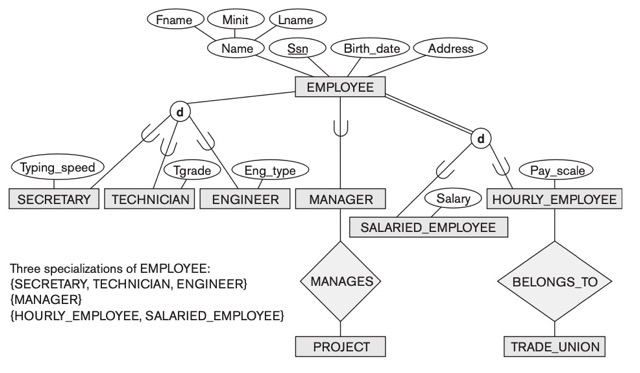
\includegraphics[scale=0.4]{gerardisg.jpeg}
\caption{Gerarchia con disjoint} 
\label{gerardisg}
\end{figure}


Per modellarlo mi chiedo quali siano le \hl{caratteristiche che hanno in comune alcune entita'}, allora tutti gli \hl{attributi in comune vanno nella superclasse}. \hl{Ogni entita' DEVE avere i suoi attributi specifici} ma non ho un attributo chiave dato che viene preso dalla superclasse.


% Graficazione superclassi e sottoclassi
\subsection{Graficazione superclassi e sottoclassi}

La graficazione avrà per:

\begin{itemize}
	\item \hl{specializzazione diretta}: si ha un segmento 
	\item \hl{gerarchia (IS-A)}: si ha un segmento con un nodo con:
		
		\begin{itemize}
			\item \textbf{d -$>$ disjoint}: NON POSSO avere un'entità che è contemporaneamente due o più sottoentità (\textbf{solo una})
			\item \textbf{o -$>$ overlap}: posso avere un'entità che è contemporaneamente due o più sottoentità (\textbf{almeno una})
			\item \textbf{U - $>$ union}: \textbf{raggruppa} entità di tipo diverso
		\end{itemize}
		
		le quali potranno avere \hl{partecipazioni totali o parziali} che indicano se la superclasse deve o meno scegliere tra le sottoclassi.
		
\end{itemize}


\begin{figure}[H]
\centering
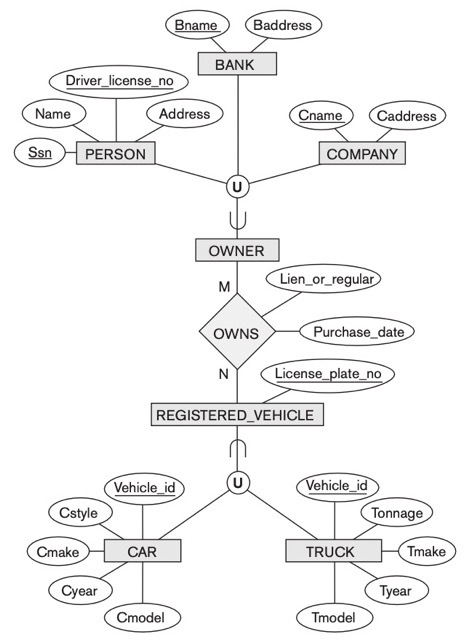
\includegraphics[scale=0.4]{union.jpeg}
\caption{Gerarchia con disjoint} 
\label{gerardisg}
\end{figure}



Il motivo della modellazione è la presenza di alcune \hl{fasi per i sistemi di gestione delle informazioni}:

\begin{itemize}
	\item studio di fattibilità
	\item analisi dei requisiti
	\item modellazione e design
	\item prototipo (ciclico)
	\item implementazione
\end{itemize}


Per i relazionali le fasi sono:

\begin{itemize}
	\item application requirements
	\item modello concettuale
	\item modello logico
	\item modello fisico
\end{itemize}


% Notazioni
\subsection{Notazioni}

Nella creazione del modello usiamo la notazione:


img notazione prof pag 7?


se sbaglio il verso delle relation metto una freccia.


Se ho bisogno di \hl{sostituire una connessione logica con un entita'} la chiamo: \hl{reificazione}. La si usa se si ha la \hl{necessita' di creare un entita' sulla quale si baseranno altre relationship}.


img pag 6


conviene usare delle relation con un nome univoco.

Se un \hl{attributo puo' avere solo un numero finito di valori} si usa: $$...[... , ...]$$


img pag 8


% Terminologia
\subsection{Terminologia}


\begin{table}[h!]
	\begin{center}
		\begin{tabular}{|c | c|} 
			\hline
			termine informale & termine formale \\ [0.5ex]
			\hline
 			table & relation \\
			column header & attribute \\
			all possible column values & domain \\
			row & tuple "<...>" \\\hline
			table definition & schema of a relation \\
			populated table & state of the relation \\
			\hline
		\end{tabular}
	\end{center}
	\caption{Tabella delle ore di lavoro}
	\label{taborelav}
\end{table}


\begin{figure}[H]
\centering
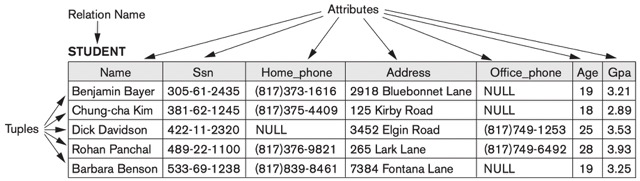
\includegraphics[scale=0.4]{termformtab.jpeg}
\caption{termini formali per le tabelle} 
\label{termformtab}
\end{figure}